\documentclass[../EngineeringJournal_CDavis.tex]{subfiles}

\begin{document}

%%%%%%%%%%%%%%%%%%%%%%%%%%%%%%%%%%%%%%%%%%%%%%%%%%%%%
%%%%%%%%%%%%%%%%%%%%%%%%%%%%%%%%%%%%%%%%%%%%%%%%%%%%%

\chapter[Configuring RIPv2]{Configuring \linebreak[1] RIPv2 \hspace*{\fill}{Jan 31, 2020}}
\noindent{{Packet Tracer Lab 7} \hspace*{\fill}{\textbf{CIT 167}}}\linebreak[1]
{{Spring 2020} \hspace*{\fill}{Chaz Davis}}                             
%===================================

\hspace{0.2cm}
\begin{tcolorbox}[width=6.3in]
\scriptsize 
- Important Commands for the Lab
  \begin{outline}
    \1 router rip 
      \2 version 2
    \1 no auto-summary
    \1 network
      \2 for when long commands are interrupted by console message
    \1 passive-interface 
  \end{outline}
\end{tcolorbox}
\hspace{0.2cm}
\normalsize  

\newpage

%===================================
\mysection{\textbf{Part 1: Configure RIPv2}}
\mysubsection{1}{Configure RIPv2 on R1}\\
I configured the Router for default rute all internet traffic through serial 0/0/1

\begin{center}
  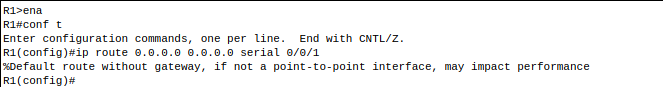
\includegraphics[scale=0.4]{Figures/2020-01-31-025239_663x87_scrot.png}
\end{center}

Next I, configured the router to use rip protocol, then to use version 2, and then passed it the no auto-summary command

\begin{center}
  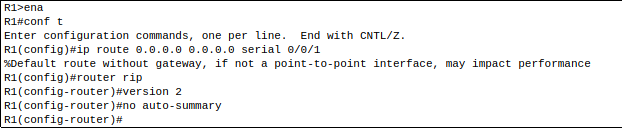
\includegraphics[scale=0.4]{Figures/2020-01-31-025628_622x128_scrot.png}
\end{center}

I set the networks on R1, and then Used the passive interface command to setup the LAN  port, and then
default-information originate to advertise the routes that I've configured see:
\ref{config7a}\subref{config7aNetSetR1}.
\hfill\break
Lastly, I stepped out of config router mode and ran the command: copy-running config
startup-config to save my work see:\ref{config7a}\subref{config7afinishR1}

\begin{figure}[!hbt]
  \begin{minipage}[c]{0.4\linewidth}
    \centering
    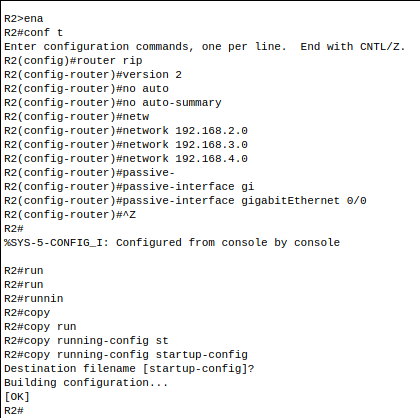
\includegraphics[scale=0.24]{Figures/2020-01-31-031204_420x418_scrot.png}
    \subcaption{setting networks R1}\label{config7aNetSetR1}
  \end{minipage}\hfill
  %
  \begin{minipage}[c]{0.4\linewidth}
    \centering
    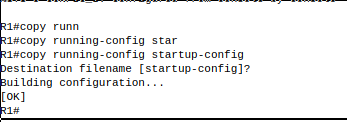
\includegraphics[scale=0.4]{Figures/2020-01-31-030648_347x122_scrot.png}
    \subcaption{Finishing up R1}\label{config7afinishR1}
  \end{minipage}
  \caption{Configuring R1 for RIPv2}\label{config7a}
\end{figure}

\mysubsection{2}{Configure RIPv2 on R2 and R3}
Next I configured R2 and R3 for their networks

\begin{figure}[!hbt]
  \begin{minipage}[c]{0.4\linewidth}
    \centering
      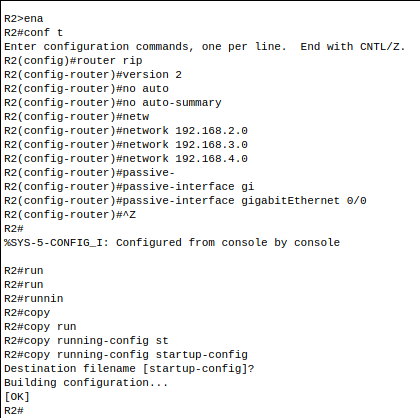
\includegraphics[scale=0.24]{Figures/2020-01-31-031204_420x418_scrot.png}
      \subcaption{Configuring R2}\label{config7bR2}
  \end{minipage}\hfill
  %
  \begin{minipage}[c]{0.4\linewidth}
    \centering
    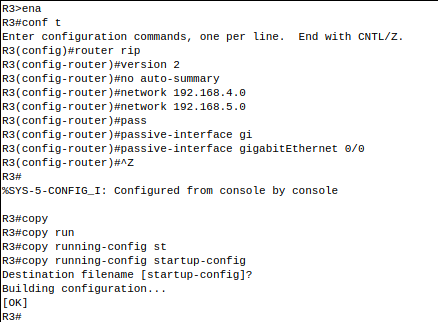
\includegraphics[scale=0.24]{Figures/2020-01-31-032105_438x322_scrot.png}
    \subcaption{Configuring R3}\label{config7bR3}
  \end{minipage}
  \caption{Configuring the Routers for RIPv2}\label{config7b}
\end{figure}

\newpage

%===================================
\mysection{\textbf{Part 2: Verify Configurations}}

\mysubsection{1}{View Routing Tables of R1, R2, and R3}

\begin{center}
  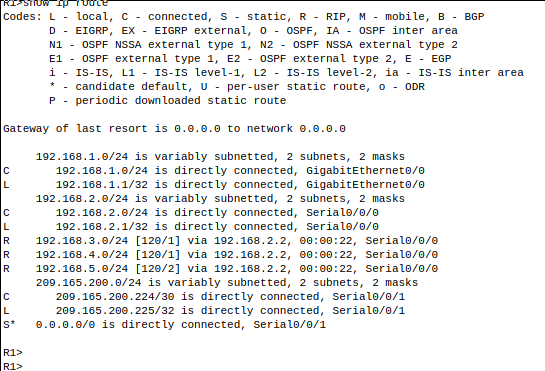
\includegraphics[scale=0.33]{Figures/2020-01-31-032604_545x371_scrot.png}
\end{center}

\begin{figure}[!hbt]
  \begin{minipage}[c]{0.4\linewidth}
    \centering
      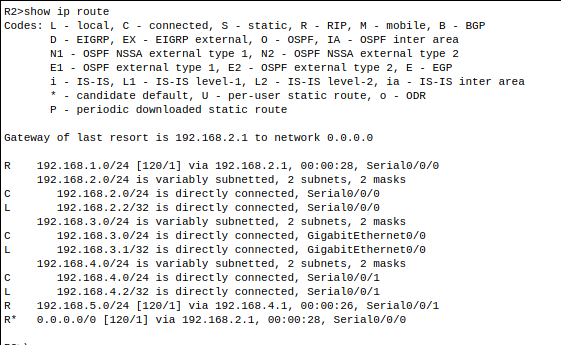
\includegraphics[scale=0.33]{Figures/2020-01-31-032658_561x345_scrot.png}
      \subcaption{Routing Tables for R2}\label{verify7R2}
  \end{minipage}\hfill
  %
  \begin{minipage}[c]{0.4\linewidth}
    \centering
    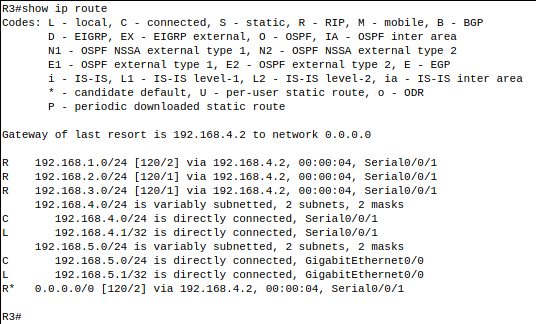
\includegraphics[scale=0.33]{Figures/2020-01-31-032725_536x324_scrot.png}
    \subcaption{Routing Tables for R3}\label{verify7R3}
  \end{minipage}
  \caption{IP Routing Tables for the Routers}\label{verify7}
\end{figure}


\mysubsection{2}{Success}

\begin{figure}[!hbt]
  \begin{minipage}[c]{0.4\linewidth}
    \centering
      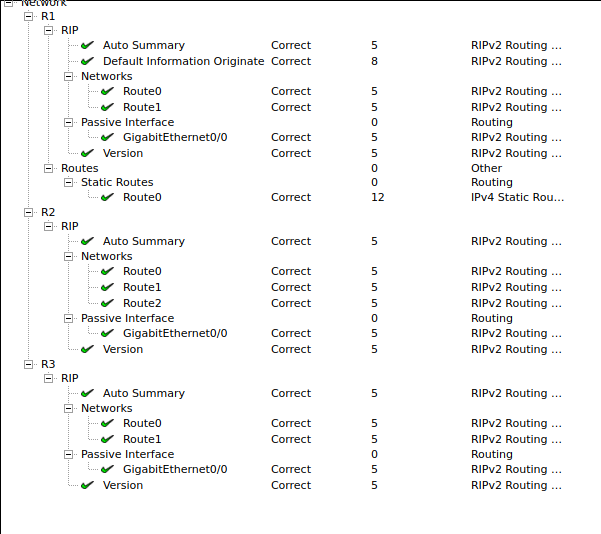
\includegraphics[scale=0.35]{Figures/2020-01-31-033357_601x534_scrot.png}
      \subcaption{Results}\label{success7result1}
  \end{minipage}\hfill
  %
  \begin{minipage}[c]{0.4\linewidth}
    \centering
    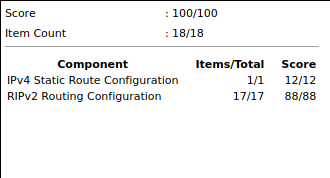
\includegraphics[scale=0.48]{Figures/2020-01-31-033406_330x178_scrot.png}
    \subcaption{All components cleared}\label{success7result2}
  \end{minipage}
  \caption{Successful Completion}\label{success7}
\end{figure}

\end{document}
